\section{Critique and Potential Improvements}
While the paper presents a very impressive method for \gls{nvs}, there are certain areas where we believe the method can improve.



% \begin{figure}
%     \centering
%     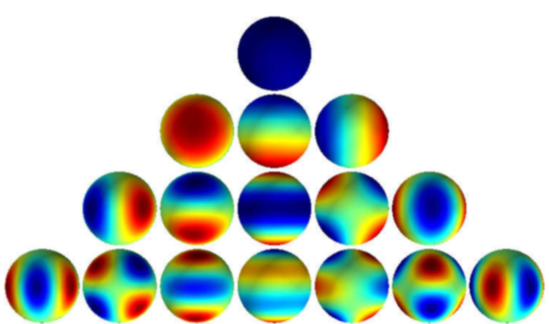
\includegraphics[width=\linewidth]{images/spherical_harmonics.png}
%     \label{fig:spherical_harmonics}
%     \caption{Visualization of the spherical harmonics used to represent the view-dependent color of each Gaussian \cite{pokorny2014a}.}
% \end{figure}

\subsection{Use CUDA Streams to increase parallelism}
The code provided by the authors showcases a deep understanding of CUDA and GPU architecture,
notably in the way they ensure memory coalescing, avoid bank conflicts and leverage shared memory in the rasterization pipeline.
This makes it surprising that they do not use CUDA streams to increase parallelism.
When training the scene on a workstation with an i9-13900KF CPU and an RTX 4090 GPU the GPU utilization was only around 30\% as the training process was severely bottlenecked by the single-threaded CPU code.
In the paper, they acknowledge that the majority (\textasciitilde 80\%) of the training time is spent in Python code, and argue it is a tradeoff to allow for easy adoption by other researchers \cite[Sec. 8]{kerbl3DGaussianSplatting2023}.
While the adaptability of the code is appreciated, it does not explain why they did not use CUDA Streams to increase parallelism, as Streams have deep support in PyTorch and can easily be disabled even if support is implemented \cite{pytorchcontributorsCUDASemanticsPyTorch2023}.

\subsection{Regularization}
The paper acknowledges that the optimized Gaussians tend to be very non-isotropic, i.e. very stretched out, as  Regularization is not performed \cite[Sec. 7.4]{kerbl3DGaussianSplatting2023}.
This is illustrated in Figure \ref{fig:very_isotropic}.
One way to solve this would be to add a cost based on the index of dispersion of the scale parameters $\bm{s}$ of each Gaussian, that is the ratio of the variance to the mean, which would have a value of 0 for spherical Gaussians.

\begin{figure}
    \centering
    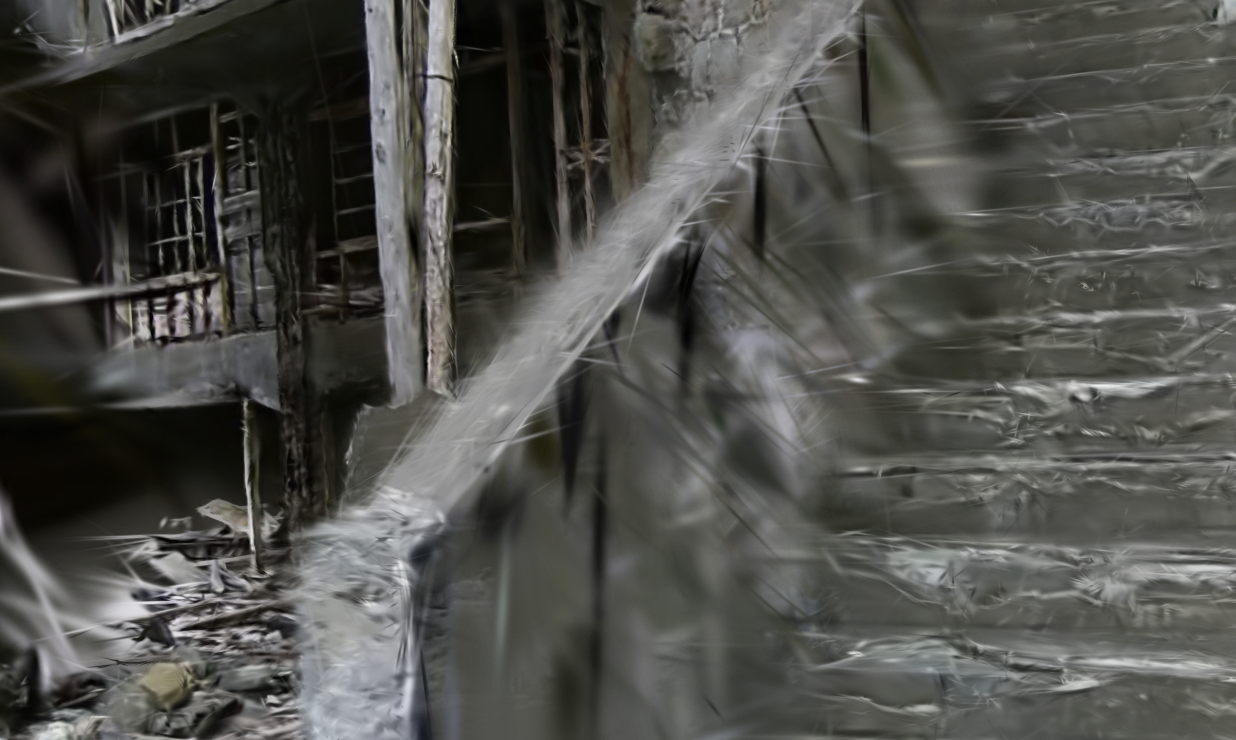
\includegraphics[width=\linewidth]{images/very_isotropic.png}
    \caption{Going outside the captured view angles illustrate how non-isotropic the Gaussians are \cite{@nekoHashimaIslandCreated2023}}
    \label{fig:very_isotropic}
\end{figure}

\subsection{Faster Opacity Calculation}
% Why they chose to use a Gaussian to represent the scene is not clearly explained in the paper.
In the current implementation, they evaluate the exponential function for each pixel for each Gaussian in the pixel's block, which is computationally expensive.
A threshold based on the Mahalanobis distance can be used to avoid this exponential calculation for most Gaussians.
\begin{align}
    m_i & =\frac{1}{2}(\bm{x}-\bm{\mu}''_i)^T \bm{\Sigma}{''}_i^{-1} (\bm{x}-\bm{\mu}''_i) \\
    a_i & =\begin{cases}
               0 \alpha_i \cdot exp(-\frac{1}{2}m_i) & \text{if } m_i \leq 3^2 \\
               0                                     & \text{if } m_i  > 3^2
           \end{cases}
\end{align}
Using a polynomial density function with shorter tails, e.g. $(1-x^2)^2$ instead of the exponential function would result in fewer tiny gradients, and avoid calling the expensive exponential function, probably resulting in a speedup.
With the current implementation being severely bottlenecked by the CPU code, this might not have a significant impact.



\subsection{Replace Spherical Harmonics}
\label{sec:spherical_harmonics}
In the current implementation, they use spherical harmonics to handle view-dependent color from reflections.
They present this approach as "following standard practice" referencing the Plenoxels and Instant Neural Graphics papers \cite{yuPlenoxelsRadianceFields2021a}\cite{mullerInstantNeuralGraphics2022}.
As the paper uses a fundamentally different representation of the scene, using the same approach for view-dependent color might not be the best choice.

The other methods both use some voxel-based representation of the scene,
where the sampling of each point is independent of the view direction,
making it necessary for each point to contain view-dependent color \cite{yuPlenoxelsRadianceFields2021a}\cite{mullerInstantNeuralGraphics2022}.
In the Gaussian splatting method, a discrete set of Gaussians is used to represent the scene, which could be leveraged to avoid the need for view dependence by having overlapping Gaussians with view-dependent opacity.
This could be used to have Gaussians that are only visible from a narrow range of view directions, placed in front of the scene geometry to simulate reflections.

The paper shows that even without spherical harmonics, the scene converges to a good result \cite[Table 3]{kerbl3DGaussianSplatting2023}.
We propose to remove the spherical harmonic coefficients from the representation of each Gaussian, reducing the parameter number from 59 to 14, altering the cost function and adding a second phase to the rendering pipeline to handle reflections.
As reflections add light to the scene, we can penalize the cost of the rendered image more if it is too dark than if it is too bright.
After convergence, we can add a second optimization step where the converged scene is kept constant and additional Gaussians with view-dependent opacity can be added to add highlights to reflective surfaces. A potential problem with this approach is however the popping effect discussed in Section \ref{sec:projection}, which makes it difficult to optimize overlapping Gaussians.